\section{評価及び考察}
本システムの識別精度を確認するため,端末を持ち上げるモーションを対象とした実験を行った.
本システムを用いてあらかじめ6名の被験者にモーションを4回入力してもらい,データの収集を行った.
各被験者ごとに,最初の3回分を登録モードにおける学習データとして用い,最後の1回分を認証モードにおける入力データとして10回認証を試行した.
また,それぞれの試行時になりすまし認証データとして筆者自身が同様のモーションを行ったデータも入力した.
識別器より得られたデータを各被験者ごとに平均したものを表\ref{auth-result}に示す.
表中の数値が低いほど端末所有者のモーション入力であると意味しており,``本人''の列では数値が低いほど良く,``なりすまし''の列では数値が高いほど良い.

結果から,被験者Eを除いて識別できているとわかる.
被験者Eについてはなりすまし認証のデータで得られた識別器の出力がより低く出ており,識別できていない.
本システムでは,端末所有者のデータとなりすまし認証によるデータを識別するためにダミーデータを用いた.
ダミーを含める割合は,増やしすぎるとなりすまし認証によるデータから得られる識別器の出力が低くなり,減らしすぎると端末所有者のデータから得られる識別器の出力が高くなるため,バランスを取る必要がある.
また,結果の良くなかった被験者Eについては終始データの変動が激しく,データの入力回数ごとで一致している部分があまり見られなかった.
これにより識別器の学習が進まず,端末所有者が入力したデータでもなりすまし認証であると識別されたのではないかと考えられる.
識別率の良かった被験者Aと良くなかった被験者Eのデータを比較したものを図\ref{compare}に示す.

\begin{figure}[!tb]
  \def\@captype{table}
  \begin{minipage}{.48\textwidth}
    \centering
    \tblcaption{識別精度の評価結果}
    \label{auth-result}
    \begin{tabular}{|c|r|r|} \hline
      \multicolumn{1}{|c|}{}  & \multicolumn{1}{c|}{本人} & \multicolumn{1}{c|}{なりすまし} \\ \hline \hline
      A & 0.346374 & 0.999796 \\ \hline
      B & 0.412742 & 0.665270 \\ \hline
      C & 0.497443 & 0.615715 \\ \hline
      D & 0.430046 & 0.618092 \\ \hline
      E & 0.730683 & 0.566426 \\ \hline
      F & 0.472196 & 0.512435 \\ \hline
    \end{tabular}
  \end{minipage}
  %
  \hfill
  %
  \begin{minipage}{.48\textwidth}
    \centering
    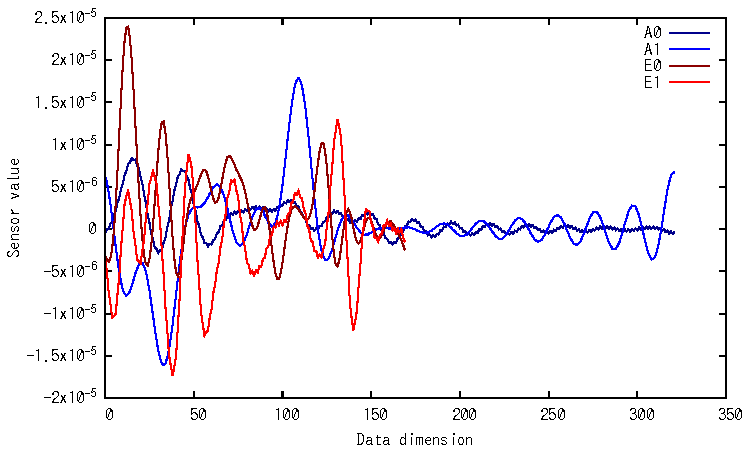
\includegraphics[bb=0 0 360 216, width=8cm]{Graphs/comp_AE.pdf}
    \caption{被験者Aと被験者Eのデータ比較}
    \label{compare}
  \end{minipage}
\end{figure}
